\chapter{The ICPC Detector Pulse-shape Library}\label{chap:library}

The ICPC pulse shape library consists of superpulses generated from radial scans at the fast and slow crystal axes with the detector at 3500\,V bias. Two 3500\,V fast axis scans were performed. The first, contemporary to the 3500\,V slow axis scan, was taken with the same camera positions, similar measurement times and before the optical noise upgrade. The second scan was taken at the end of the data taking campaign with slightly different camera positions and increased measurement times. This was done to increase statistics, specifically in the lower regions on the detector. This chapter shows the results for the high-statistics fast axis scan, which produced less noisy pulse shapes. However, the first 3500\,V fast axis scan has the advantage of being performed with the same camera positions as the 3100\,V scans, a feature that was exploited in Chapter~\ref{chap:trapping}. The high-statistics scan consists of 15 days of data, whereas the other scans consist of half this live time. For the two axes listed, results are organized in three types of plots:
\begin{itemize}
	\item Cut survival and number of events: the $AvsE$ and self-similarity cut survival fractions are shown for each voxel. As Chapter~\ref{chap:pipeline} describes, these cuts are applied sequentially, with the self-similarity cut acting only on events passing the $AvsE$ cut. In these plots the number of 2-hit self-similar events is shown. From this population a base superpulse is constructed, and all 1-hit events with $\chi^2/\text{ndf}$ join the 2-hit self-similar events to form a final superpulse. Occasional excesses in the number of events were caused by errors in data taking. At such radii data were retaken. The errored data were later recovered, leading to the excess. 
	\item Rise time and current amplitude ($A$): The 0.3-99.7\% rise time and current amplitude is calculated from the superpulses and shown in their corresponding voxels. The same procedure is carried out for simulated superpulses and the results are shown on the right of the counterparts from data. For ease of comparison between axes and biases, and data and simulation, the color axes for all configurations are normalized to the same values. 
	\item Waveforms: Superpulses from data and simulation are shown for a select number of voxels at a given $r$ on the top and bottom respectively. The selected voxels, labeled with the same color as the superpulses are shown on the pictogram of the figure. A plot showing the number of 2-hit self-similar events on which each superpulse was built is included on the top left of each figure. In combination with the self-similarity survival, this plot provides a degree of reliability for each superpulse from data. As a heuristic, voxels with less than 5 self-similar hits or a self-similarity survival below 50\% (depicted in blue in the self-similarity cut survival plots) are not considered reliable. 
\end{itemize}

The radial scans were performed along the crystal axes determined by the \BaS{} scan presented in Sec.~\ref{sec:crystal_axis_Ba}. Analysis of Compton data from an azimuthal scan at the outer edge of the detector later found that these crystal axes could be incorrect by be approximately 3.1$^\circ$. This chapter starts with a discussion of this discrepancy, and includes the results from Compton data. The results from the radial scans at operational and near operational voltage follow.

\section{Crystal Axis Determination from Compton Events}\label{sec:crystal_axis_Cs}

The ICPC was scanned in the $\phi = [4.9, 94.9]^\circ$ range every $5^\circ$ at $r = 34.4$\,mm. This radius was chosen such that just over half of the \CsS{} beam was contained within the active volume of the detector. The result is that most Compton scattered gammas originate from the outer edge of the active volume, similar to where the 81\,keV \BaS{} gammas were deposited. In this manner, the anisotropies are expected to match at a reconstructed $z$ matching the $z$-position of the \BaS{} source. The number of events used to build the superpulses, and the 1-99\% rise times for each voxel are shown in Fig.~\ref{fig:Cs_crystal_axis}.
\begin{figure}[htb]
    \centering
    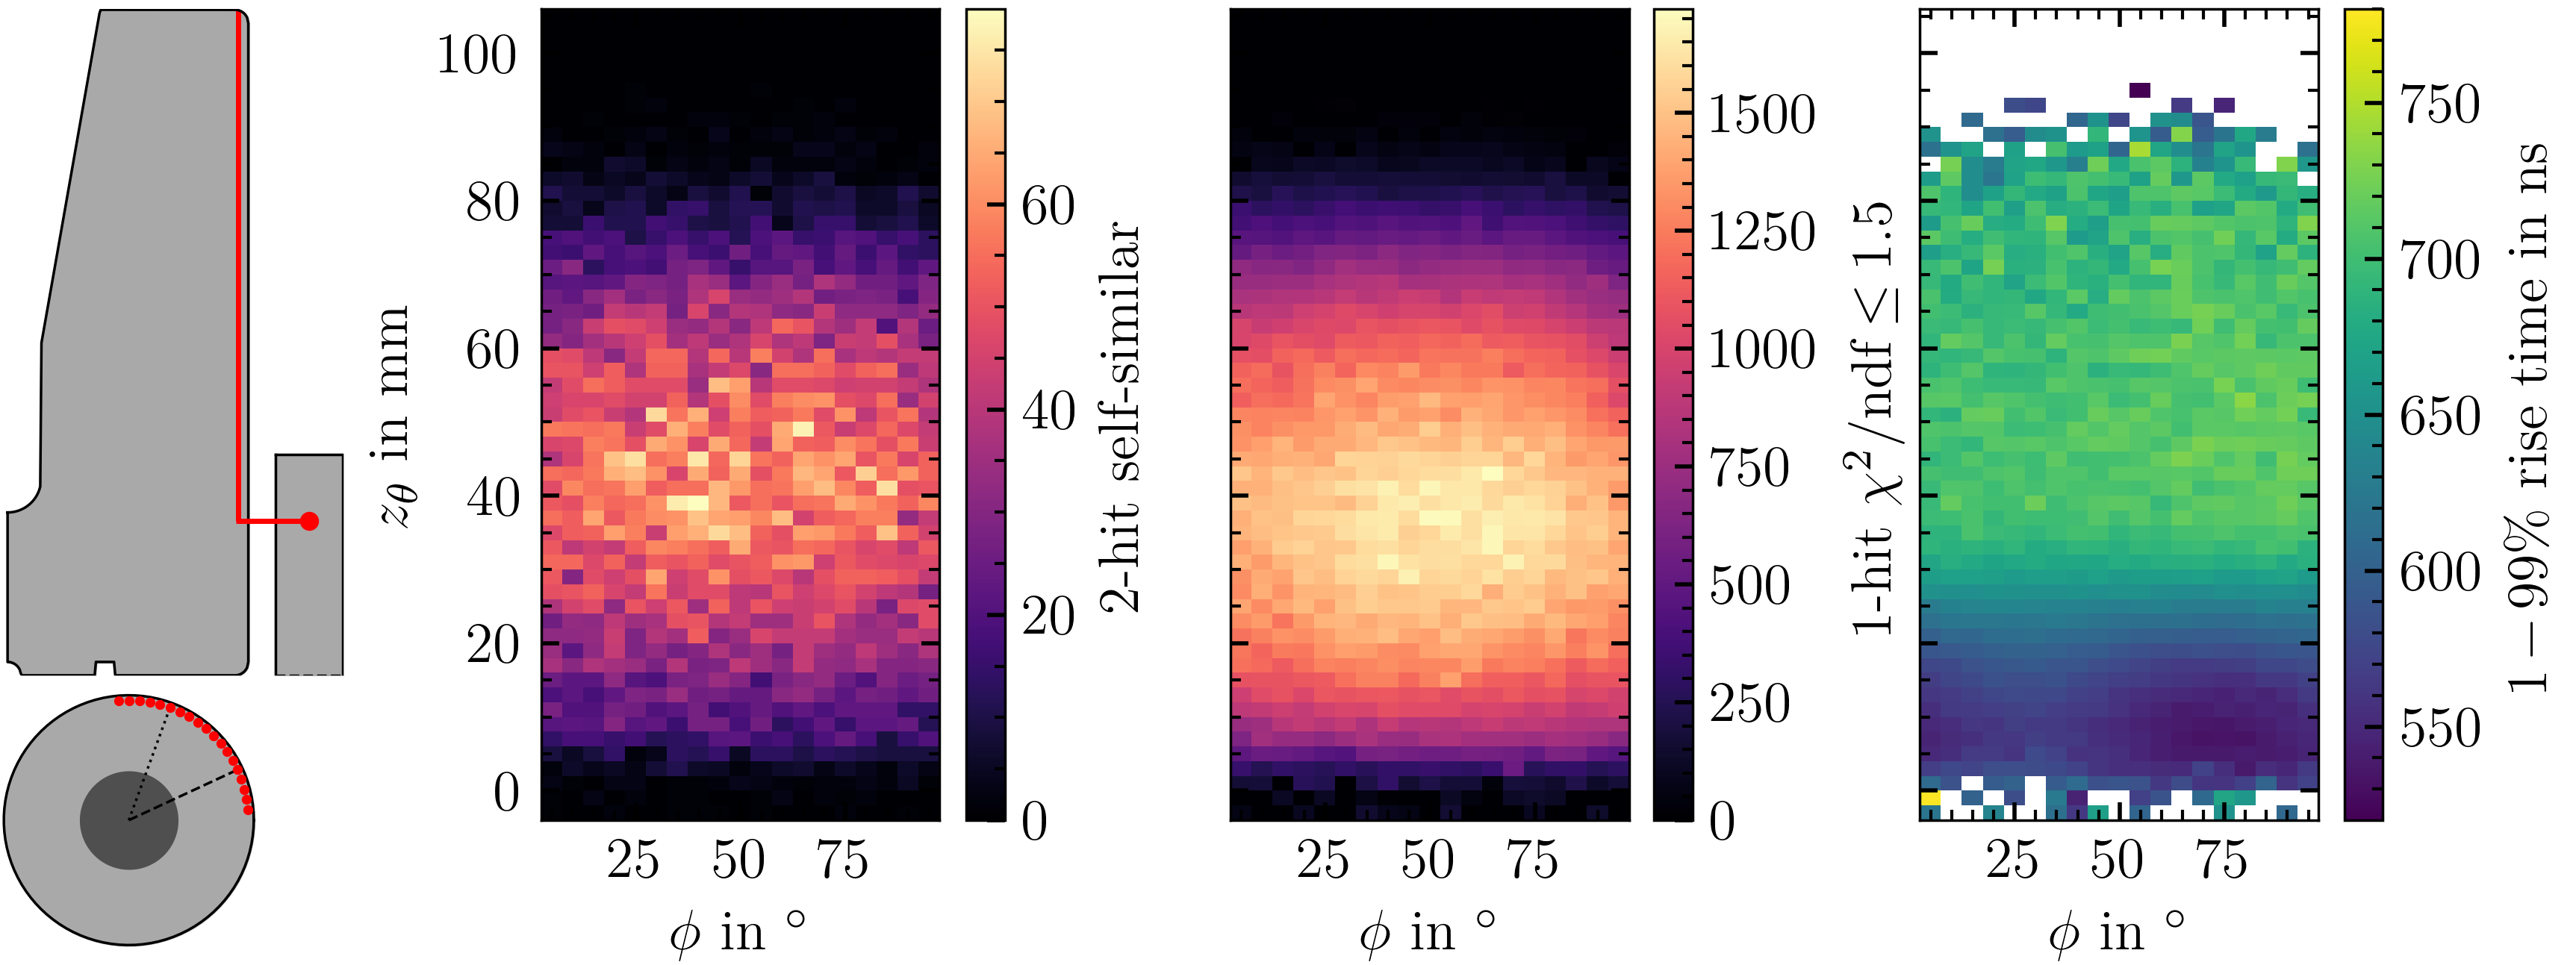
\includegraphics[width=6in]{figs/library/Cs_crystal_axis.png}
    \caption{The number of 2-hit self-similar events and 1-hit events used to build the superpulses are shown on the left and middle respectively for voxels at all $\phi$ in the azimuthal scan at $r = 34.4$\,mm. From these superpulses, the 1-99\% rise time is calculated and shown on the right.}
    \label{fig:Cs_crystal_axis}
\end{figure}
A simultaneous fit to the 1-99\% rise time is performed at all reconstructed $z$. The result of this fit is shown in Fig.~\ref{fig:Cs_crystal_axis_fits} for the lower quarter of the detector. Note that anisotropy is lost above 25\,mm, at the same height as where the borehole begins. 

An anisotropy of $16.3\pm1.5$\,ns was found at $z = (5\pm1)$\,mm, which agrees (within error) with the \BaS{}-data anisotropy ($(18\pm0.9)$\,ns at $z = (4.3\pm1.6)$\,mm). The simultaneous fit determines a slow axis position of $(28.1\pm0.2)^\circ$, which is in slight tension with the \BaS{} result: $(24.9\pm1.6)^\circ$. The difference can be in part attributed to the slight center misalignment and drift. This effect is observed in Fig.~\ref{fig:Cs_crystal_axis}, where the maximum number of counts occurs in the $\phi = [35, 55]^\circ$ range. This is consistent with the center misalignment parameters calculated in Sec.~\ref{sec:centeralignment}, where $\Delta A = (39.7\pm1.2)^\circ$.
\begin{figure}[H]
    \centering
    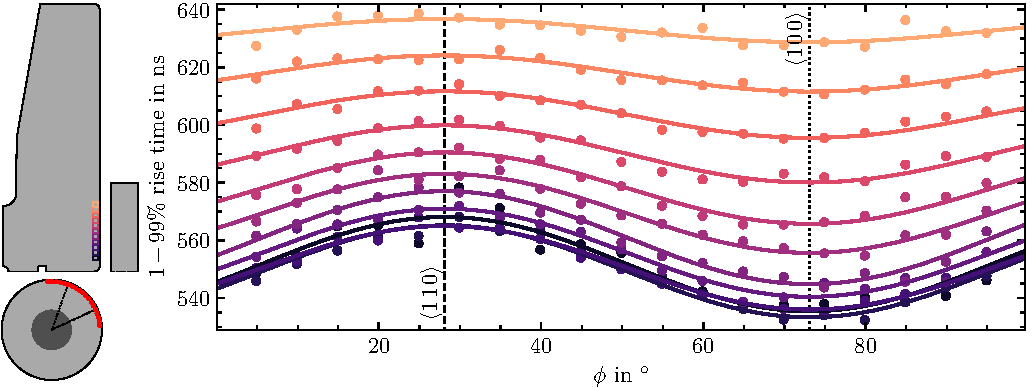
\includegraphics[width=6in]{figs/library/Cs_crystal_axis_fits.pdf}
    \caption{The 1-99\% rise times from the rightmost panel of Fig.~\ref{fig:Cs_crystal_axis} are shown as a scatter plot for $z = [5, 25]$\,mm. Darker colors represent lower $z$-values as the pictogram depicts. The simultaneous fit performed in the aforementioned $z$-range results in the sinusoidal functions drawn for each $z$.}
	\label{fig:Cs_crystal_axis_fits}
\end{figure}

\clearpage

\section{Fast Axis}
\begin{figure}[H]
    \centering
    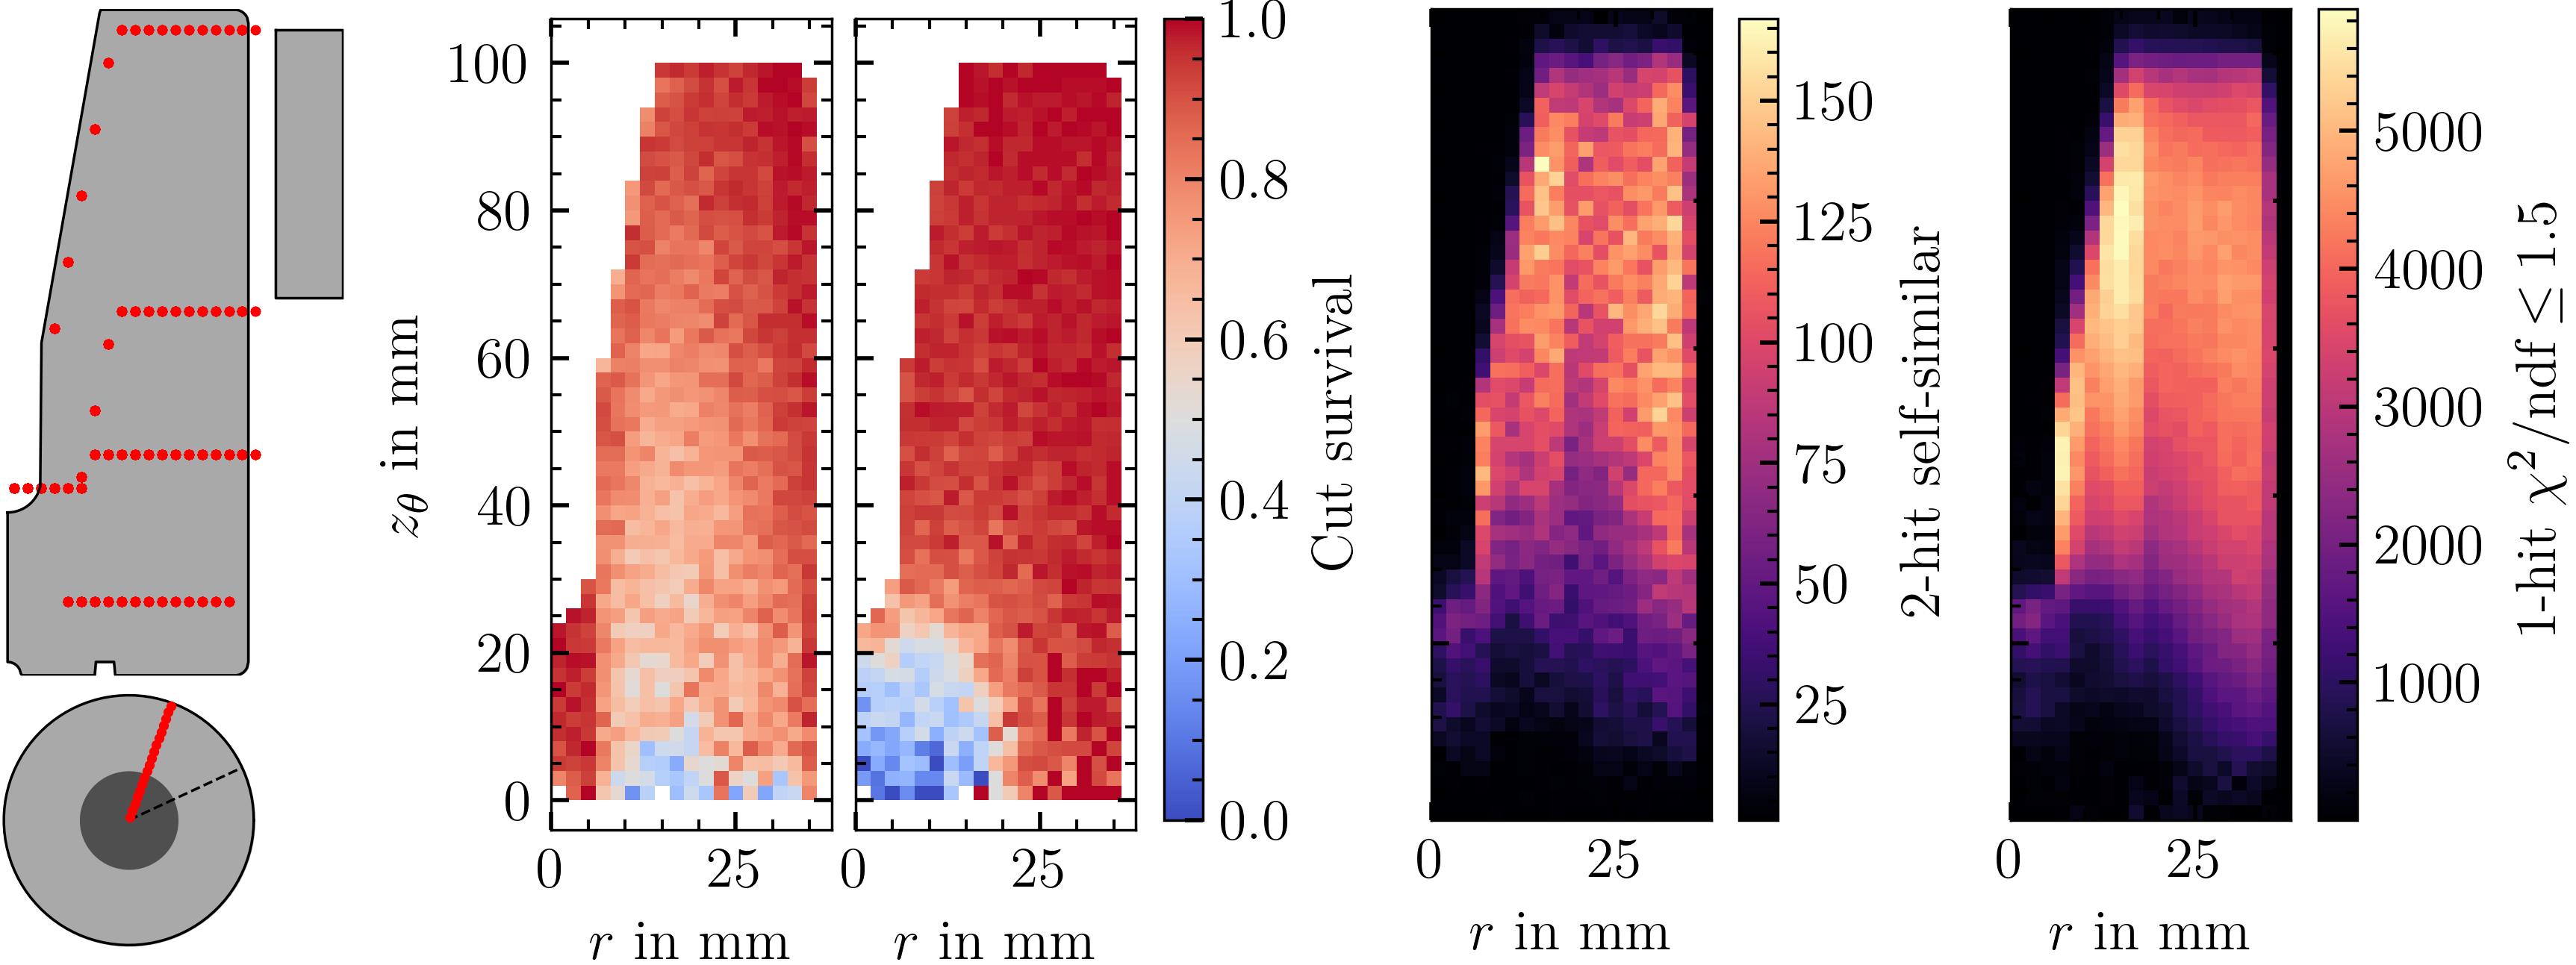
\includegraphics[width=6in]{figs/library/fast_axis_nhits.png}
    \caption{The 2-hit survival fractions of the successive application of the $AvsE$ and self-similarity cuts are shown in the first and second panel respectively for the $\left<1\,0\,0\right>$-axis scan at 3500\,V. The number of 2-hit self-similar events and 1-hit events used to build the superpulses are shown in the third and fourth panel respectively.}
	\label{fig:fast_axis_nhits}
\end{figure}
\begin{figure}[H]
    \centering
    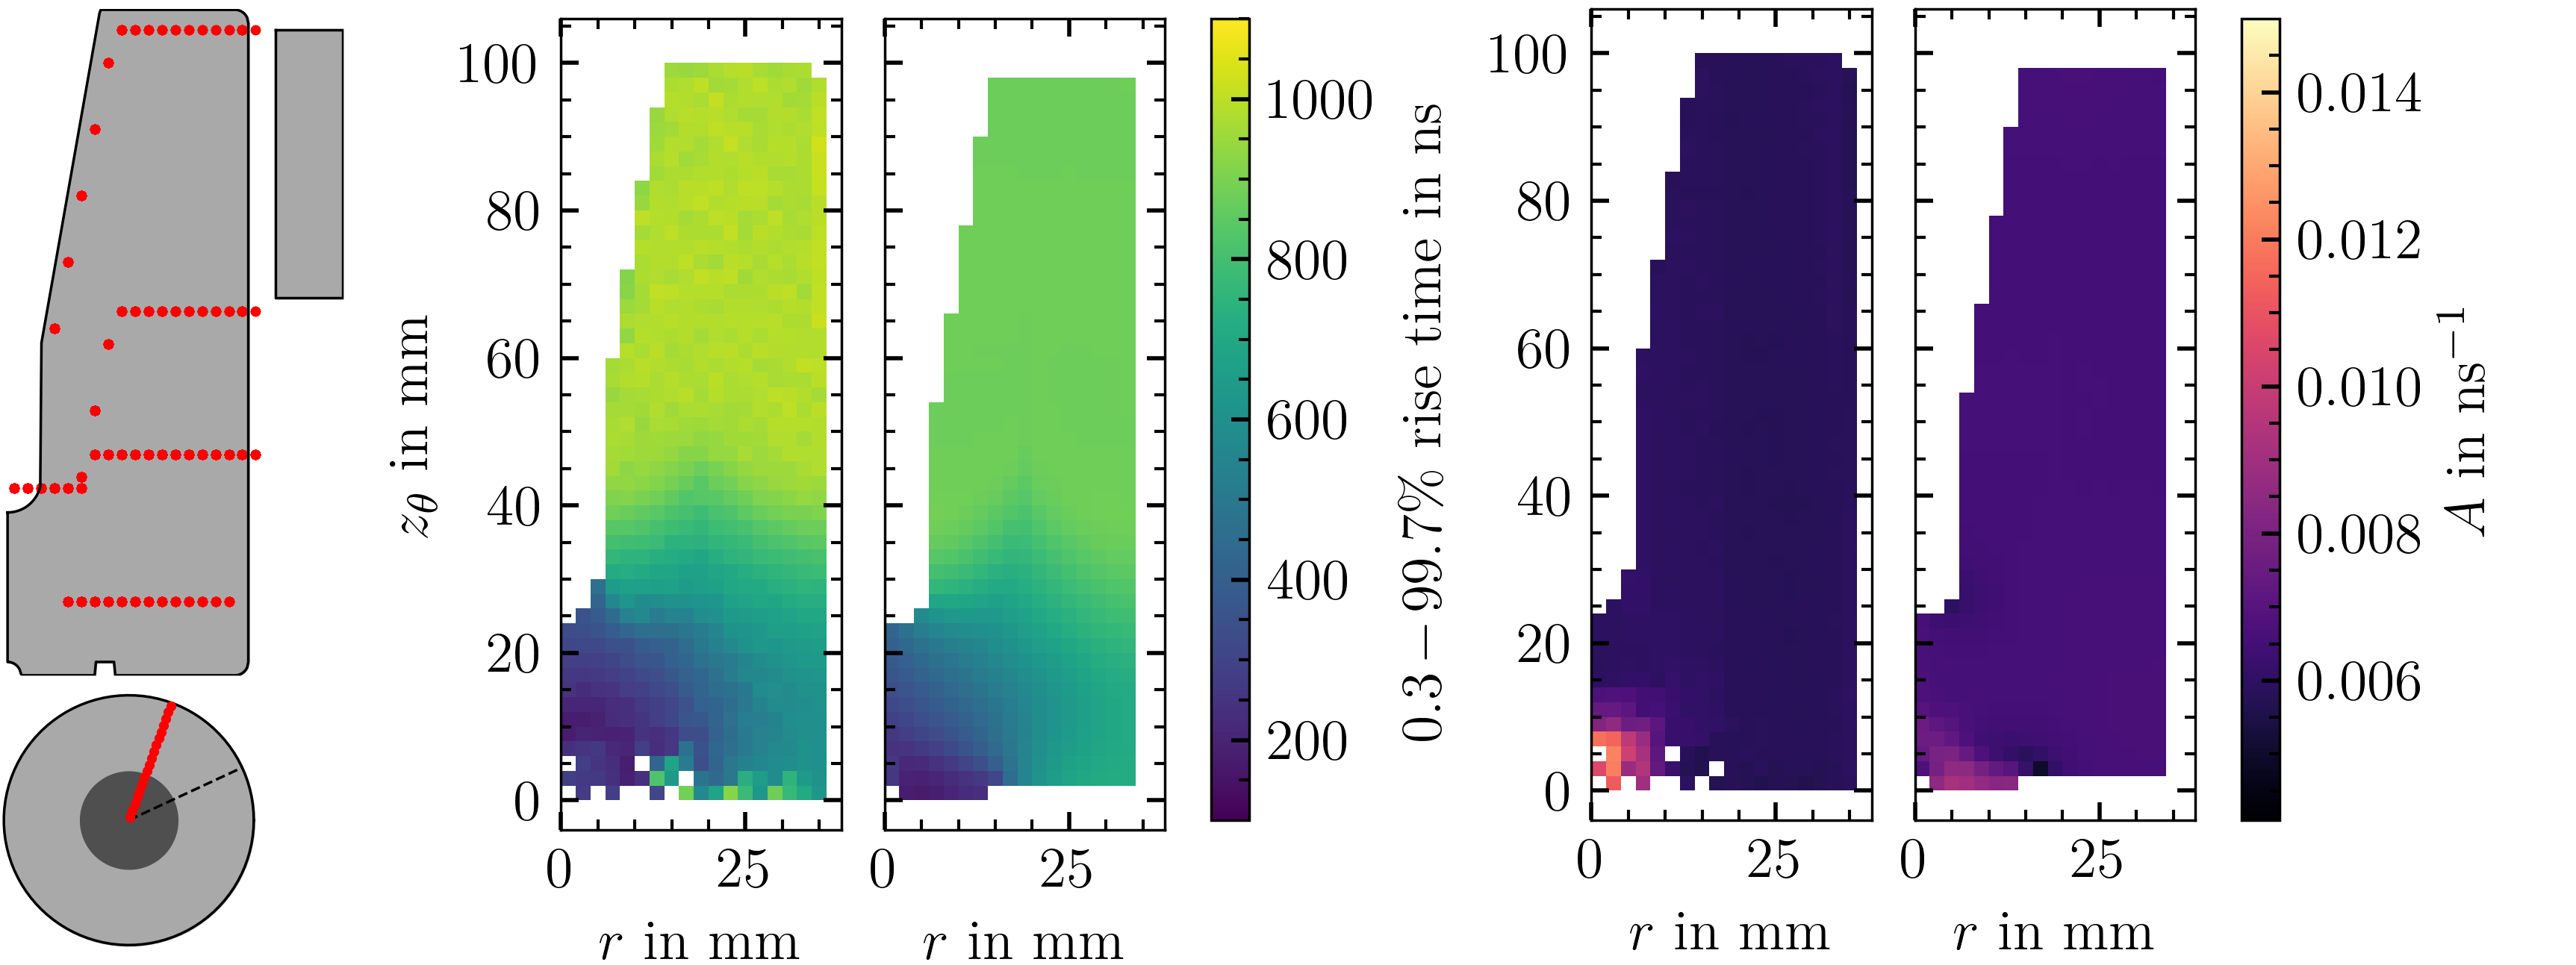
\includegraphics[width=6in]{figs/library/fast_axis_dt_aoe.png}
    \caption{The specified rise times from data and simulated superpulses are shown in the first and second panel respectively for the $\left<1\,0\,0\right>$-axis scan at 3500\,V. The $A$ calculated from data and simulated superpulses are shown in the third and fourth panel respectively.}
	\label{fig:dt_aoe_fast_axis}
\end{figure}

\begin{figure}[H]
    \centering
    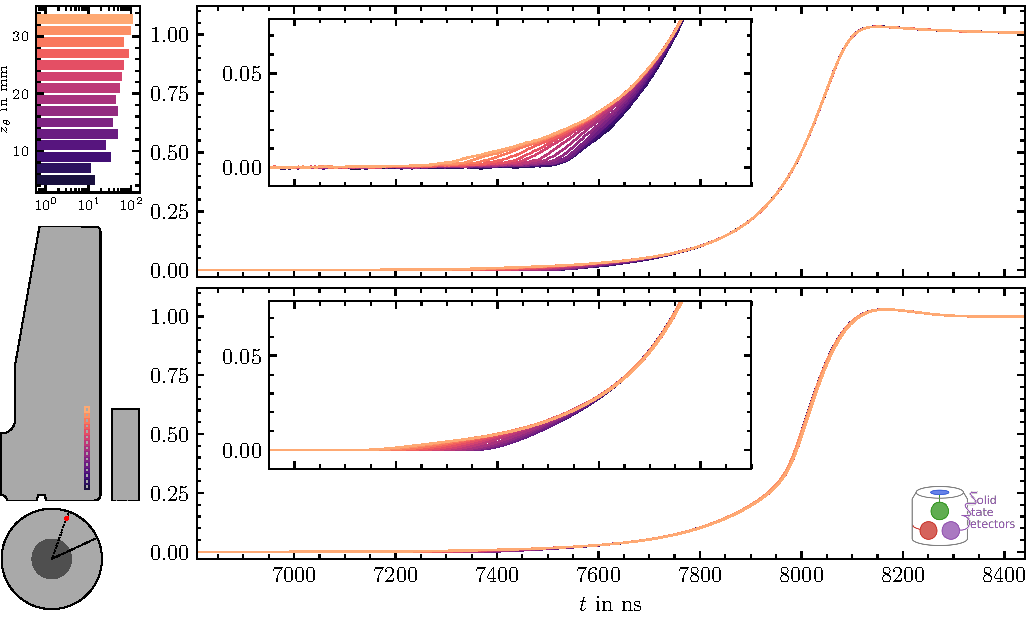
\includegraphics[width=6in]{figs/library/fast_axis_r_31_pulses.pdf}
    \caption{The $(r = 31, z = [5,33])$\,mm, $\left<1\,0\,0\right>$, HV = 3500\,V superpulses are depicted, with an inset (with matching $x$-scale) showing a close up of the start of the rise.}
\end{figure}
\begin{figure}[H]
    \centering
    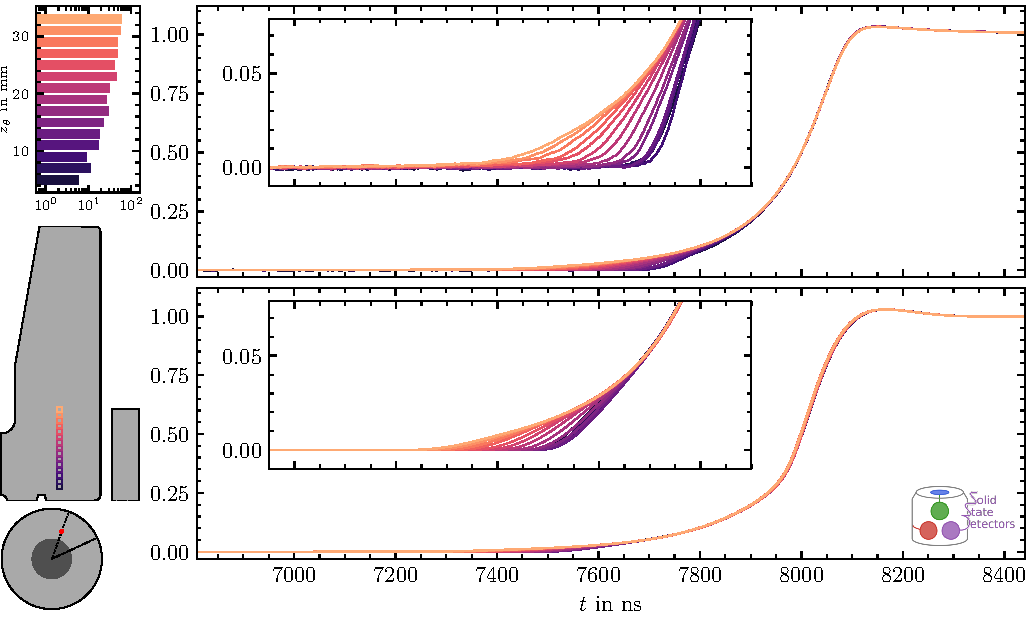
\includegraphics[width=6in]{figs/library/fast_axis_r_21_pulses.pdf}
    \caption{The $(r = 21, z = [5,33])$\,mm, $\left<1\,0\,0\right>$, HV = 3500\,V superpulses are depicted.}
\end{figure}


\section{Slow Axis}

\begin{figure}[H]
    \centering
    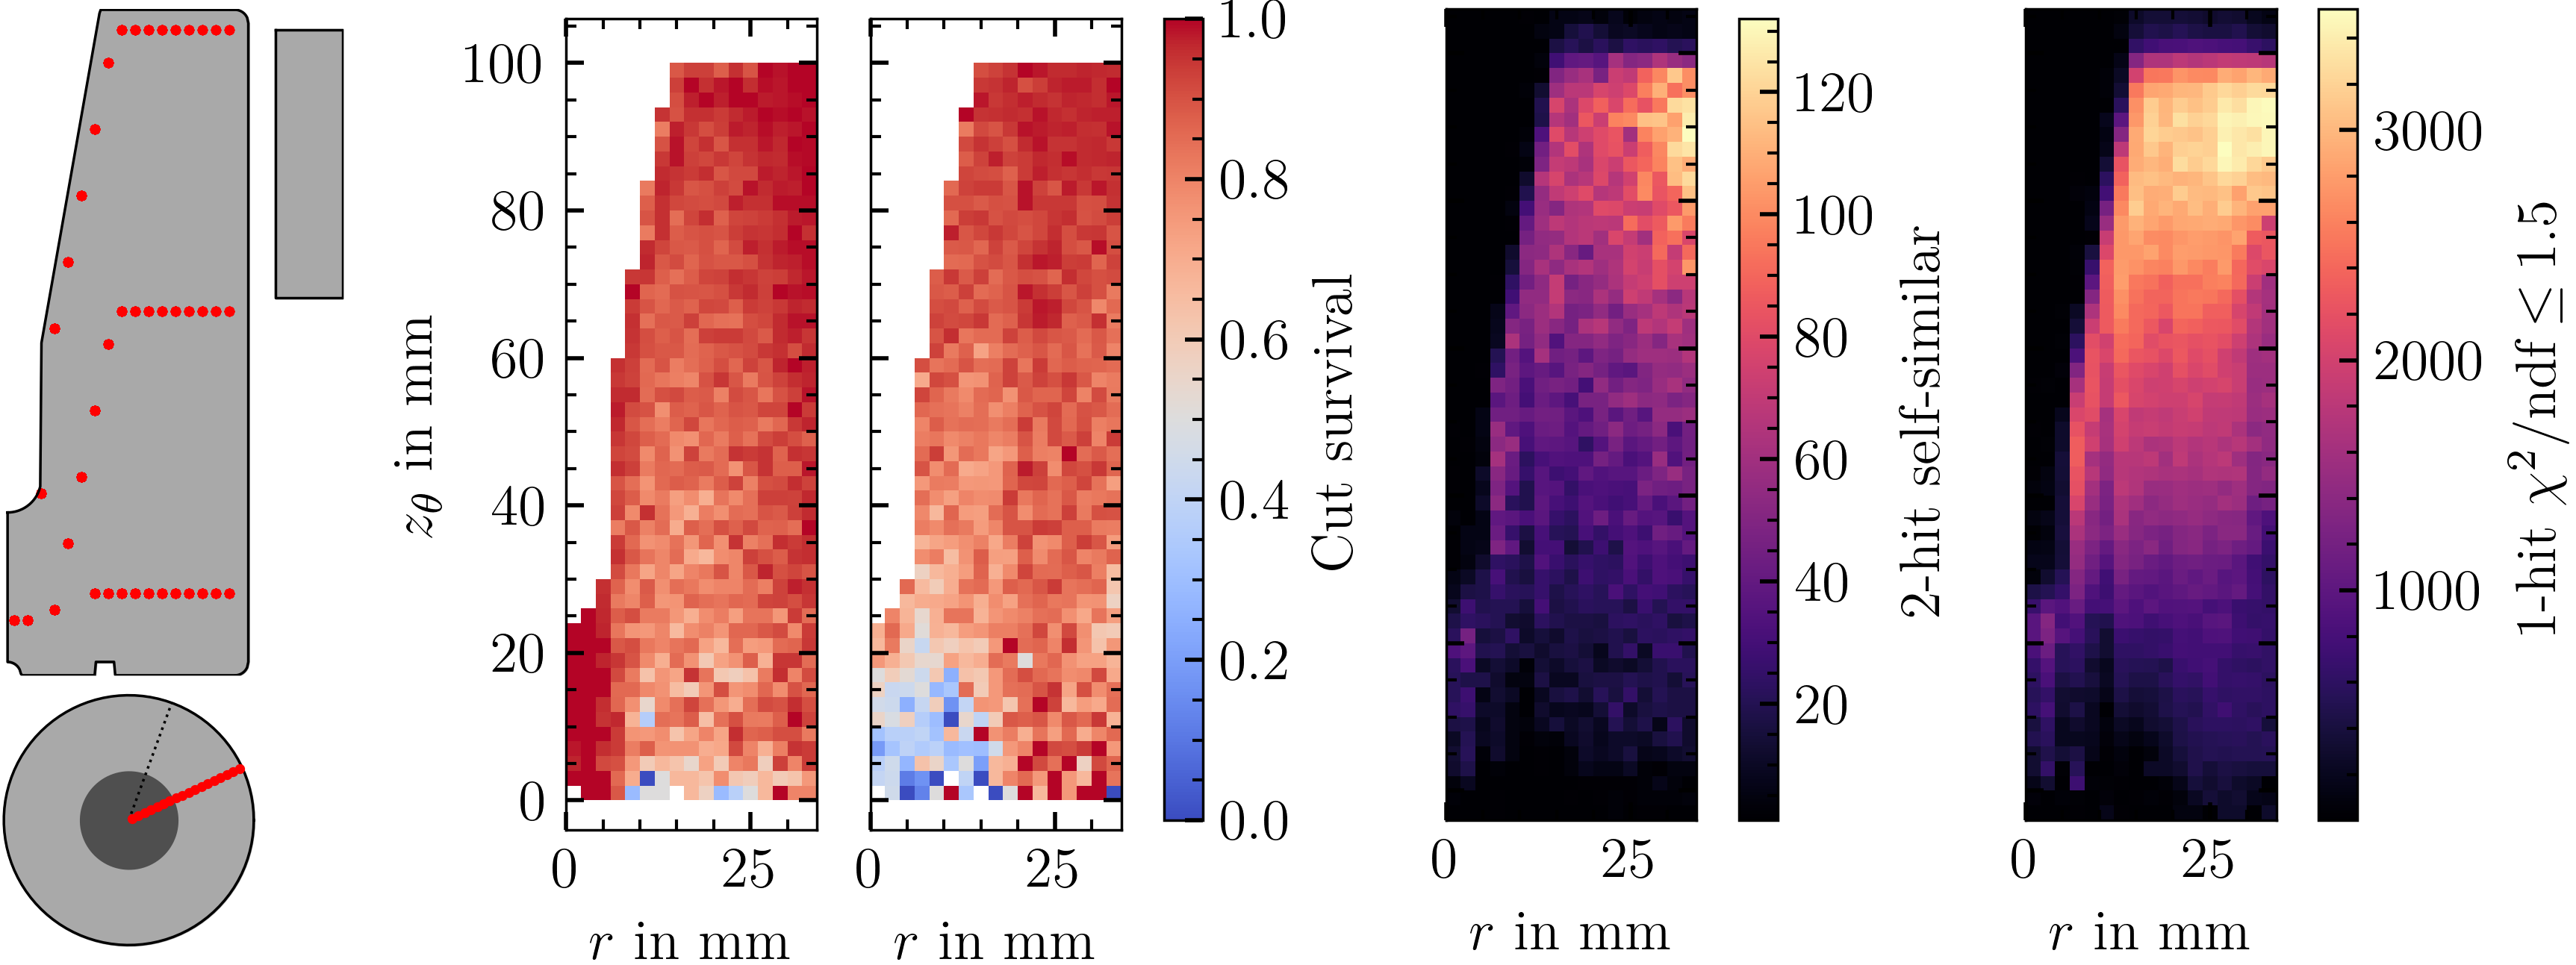
\includegraphics[width=6in]{figs/library/slow_axis_nhits.png}
    \caption{The 2-hit survival fractions of the successive application of the $AvsE$ and self-similarity cuts are shown in the first and second panel respectively for the $\left<1\,1\,0\right>$-axis scan at 3500\,V. Due to the high noise levels prior to the optical upgrade, the self-survival cut survival is considerably lower overall than the high-statistics $\left<1\,0\,0\right>$-axis scan. Additionally, $AvsE$ is bimodal, leading to a poor single-site cut performance. The number of 2-hit self-similar events and 1-hit events used to build the superpulses are shown in the third and fourth panel respectively.}
	\label{fig:slow_axis_nhits}
\end{figure}
\begin{figure}[H]
    \centering
    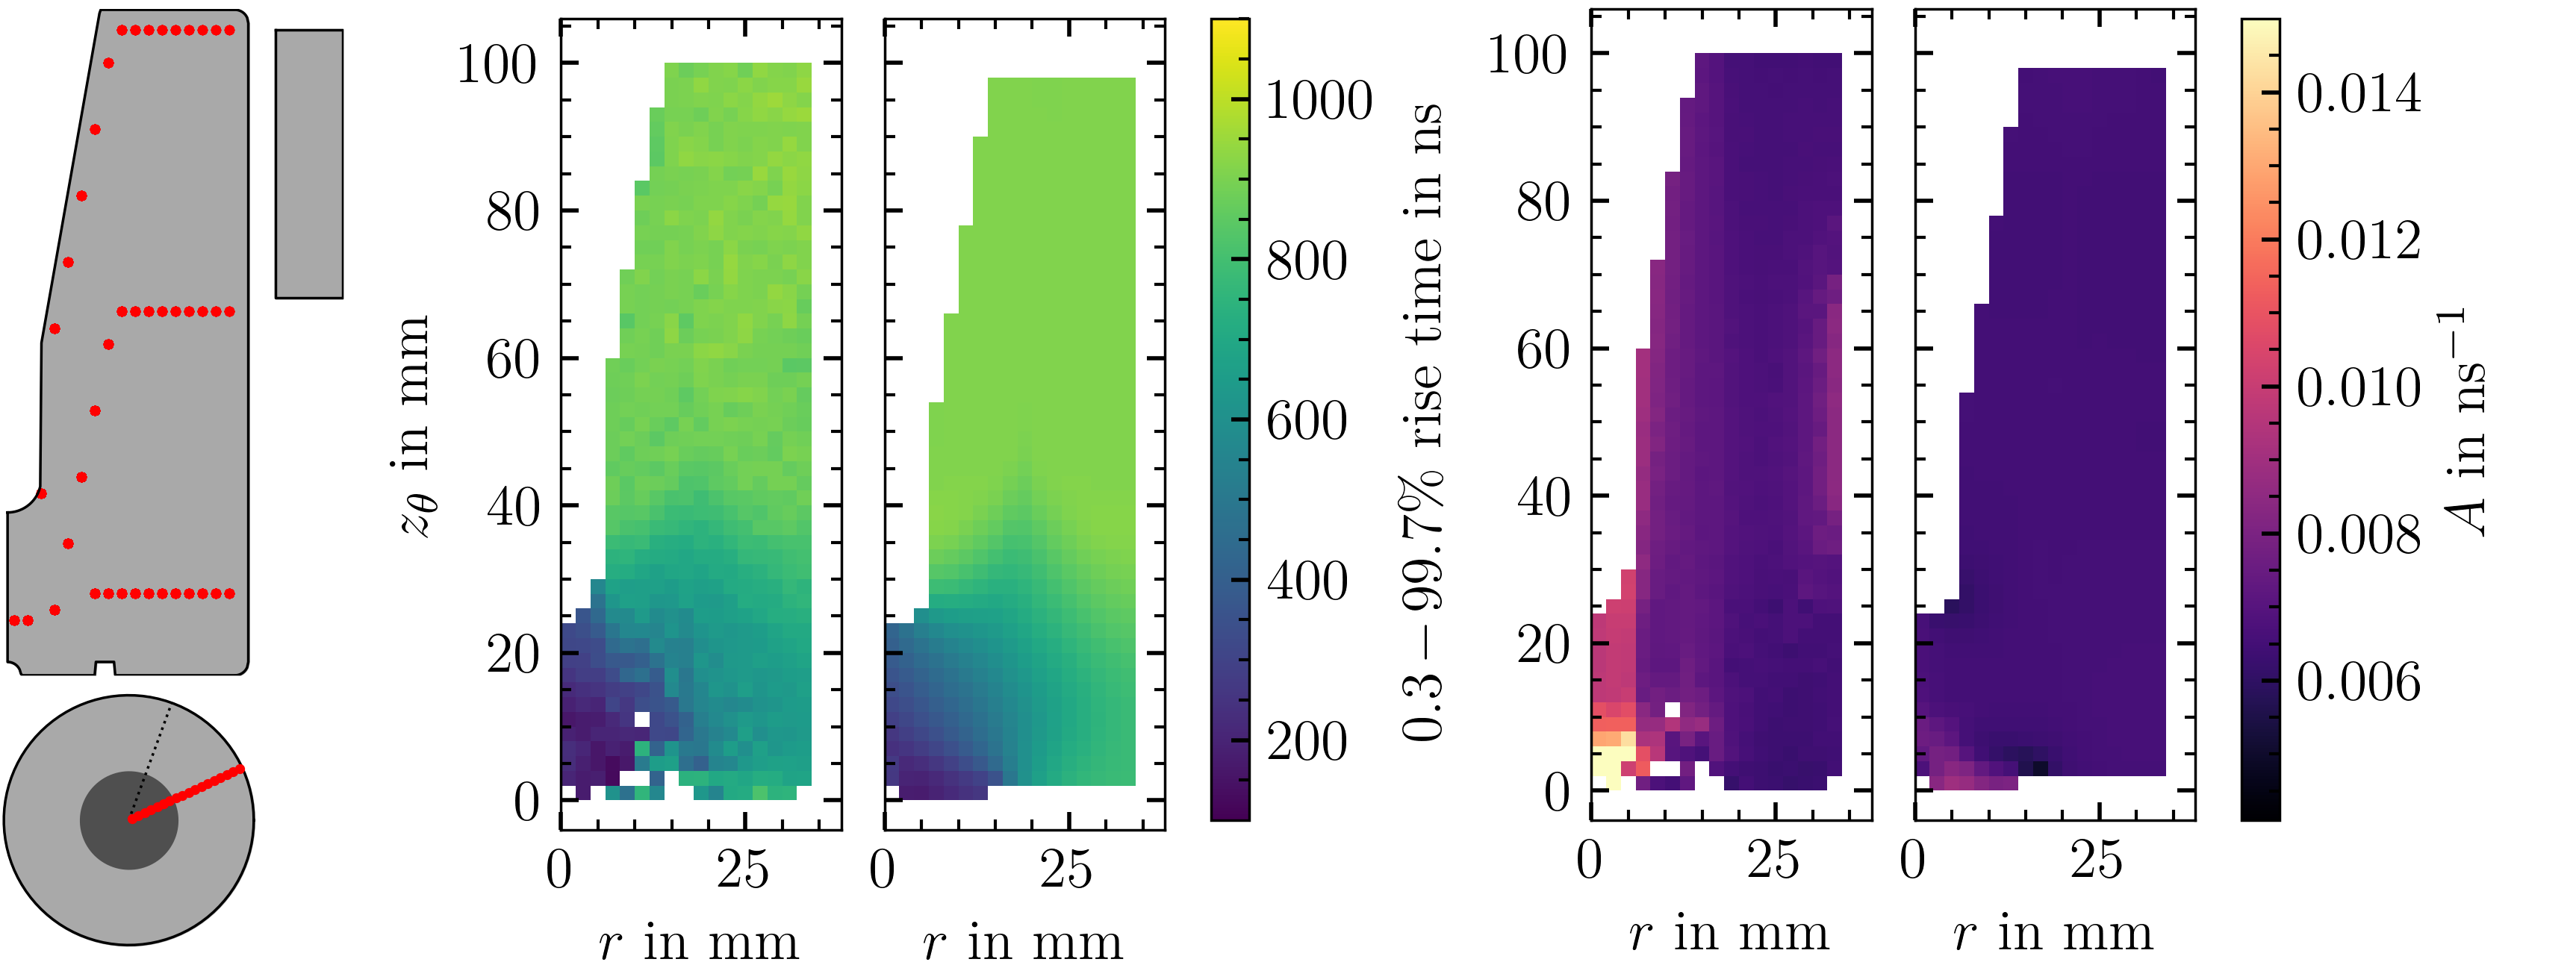
\includegraphics[width=6in]{figs/library/slow_axis_dt_aoe.png}
    \caption{The specified rise times from data and simulated superpulses are shown in the first and second panel respectively for the $\left<1\,1\,0\right>$-axis scan at 3500\,V. The $A$ calculated from data and simulated superpulses are shown in the third and fourth panel respectively. The measured $A$ is unstable due to the high noise levels prior to the optical upgrade.}
	\label{fig:dt_aoe_slow_axis}
\end{figure}

\begin{figure}[H]
    \centering
    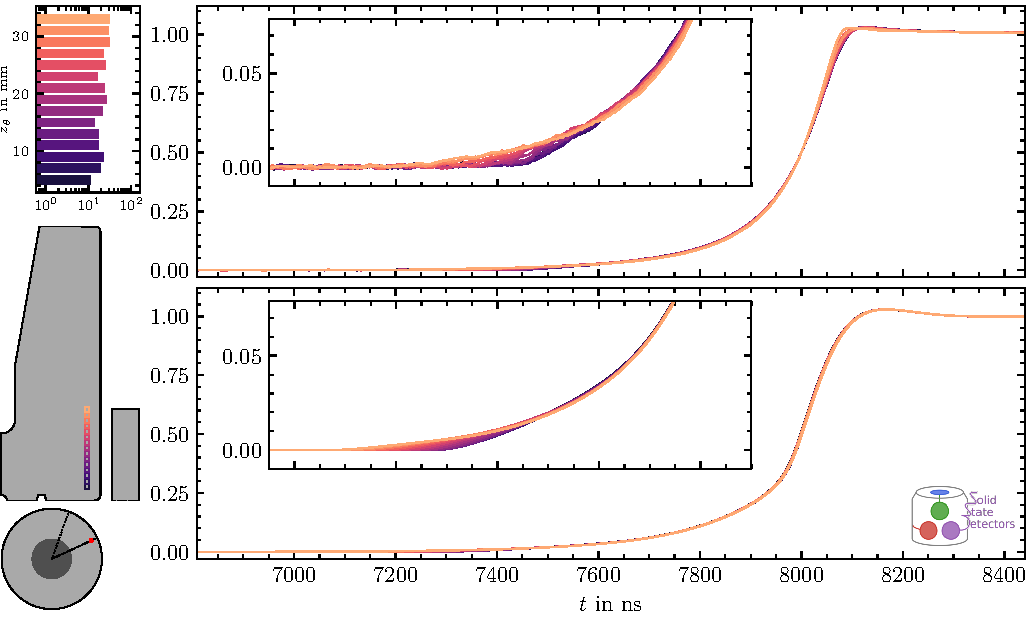
\includegraphics[width=6in]{figs/library/slow_axis_r_31_pulses.pdf}
    \caption{The $(r = 31, z = [5,33])$\,mm, $\left<1\,1\,0\right>$, HV = 3500\,V superpulses are depicted, with an inset (with matching $x$-scale) showing a close up of the start of the rise.}
\end{figure}
\begin{figure}[H]
    \centering
    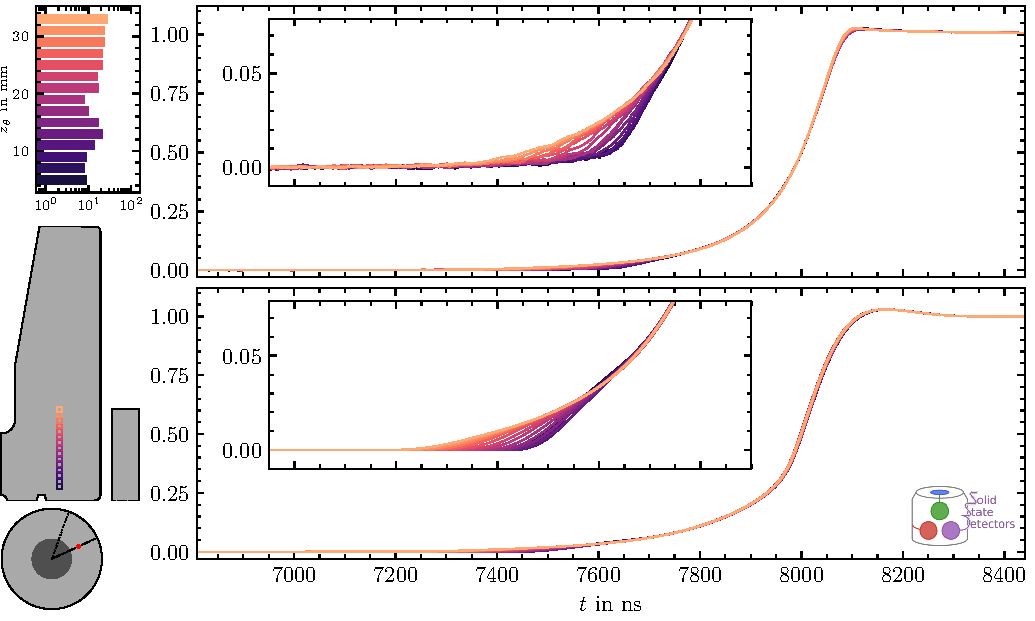
\includegraphics[width=6in]{figs/library/slow_axis_r_21_pulses.pdf}
    \caption{The $(r = 21, z = [5,33])$\,mm, $\left<1\,1\,0\right>$, HV = 3500\,V superpulses are depicted.}
\end{figure}

\section{Discussion}
The data from the azimuthal scan shown in Sec.~\ref{sec:crystal_axis_Cs} were taken contemporary to the high statistics fast axis data. As expected, the 1-99\% rise times of the fast axis radial scan are consistent with those in the azimuthal scan taken at the same position. The same, however, cannot be said about slow axis data, which were taken well before the optical upgrade. Note that this upgrade included changes to the grounding scheme. The first hint of poor pre-upgrade data quality comes from the $AvsE$ cut survival in Fig.~\ref{fig:slow_axis_nhits}. Here, an abnormally high cut survival can be seen. Inspection of these distributions, and all others taken before the upgrade revealed a bimodal $AvsE$. This is reflected in Fig.~\ref{fig:dt_aoe_slow_axis}, where $A$ is notably unstable. Ripple effects of this instability can be seen in the other heatmaps. A region of high measured $A$ values in the outer edge of the detector matches that of an underfluctuation in the number of 1-hit events passing the $\chi^2/\text{ndf}\le1.5$ cut. Furthermore, the 2-hit self-similarity survival is lower compared to that of the fast axis scan. Finally, the slow axis 0.3-99.7\% rise times are lower that of the fast axis, showing that the noise upgrade had a significant impact on this parameter. 

The electronics response function was measured before and after the optical upgrade. Besides an overall reduction of noise in the individual pulses used to construct the electronics response superpulse in the post-upgrade data, no differences were found. Thus, the upgrade did not affect the electronics response to pulsed signals. Meanwhile, the upgrade resulted in increased rise times and decreased $A$ for real signals. This proves the statement previously made about the measured electronics response function for this system: it does not model the effect of the electronics on real signals. 

Fast axis data quality is excellent. $A$ is extremely stable, and as demonstrated in Sec.~\ref{subsec:singlesitecompton}, a good $AvsE$ performance is achieved. Close to the point contact, the self-similarity cut survival drops drastically to below 50\%. This is due to the high weighting potential in the region, which leads to pulse shapes which differ significantly within a voxel. Therefore, misreconstructed pulses cannot be removed with the self-similarity technique. ICPCs with BEGe-like p$^+$ contacts are expected to be less prone to this issue, given that their weighting potential is less localized. The inability to construct reliable superpulses close to the point-contact is unavoidable; however, improving the position resolution can result in smaller affected regions, given that smaller voxel sizes could be used. Additionally, information from these voxels is still valuable. Since they contain correctly reconstructed pulses, the overall trends in rise time match those from simulation. Pulse shape trends for the entire radial slice match as well. The differences in individual measured and simulated pulses stem from the uncertainties in simulation given at the end of Sec.~\ref{sec:impcomp}.

The fast axis data can used as a reliable measured pulse shape library. This statement is applicable to the red voxels satisfying $z \ge 3$\,mm in the second panel of Fig.~\ref{fig:slow_axis_nhits}, which cover most of this radial slice of the detector. In these voxels there is high enough statistics and self-similarity cut survival to lend a high degree of credibility to the calculated pulse shapes.